\documentclass[a4paper,14pt]{extarticle} 
\usepackage[a4paper,top=1.5cm, bottom=1.5cm, left=2cm, right=1cm]{geometry}
%\usepackage[T2A]{fontenc}
%\usepackage[english, russian]{babel}
\usepackage{graphicx}
\DeclareGraphicsExtensions{.pdf,.png,.jpg}

\usepackage{fontspec}
\setmainfont{Times New Roman}
\setsansfont{FreeSans}
\setmonofont{FreeMono}
\renewcommand{\baselinestretch}{1.5}
\usepackage{polyglossia}
\setdefaultlanguage{russian}
\setotherlanguages{english,russian}
\usepackage{setspace}
\usepackage[many]{tcolorbox}

\begin{document}
    \begin{center}
        \thispagestyle{empty}
        \begin{singlespace}
        МИНИСТЕРСТВО ЦИФРОВОГО РАЗВИТИЯ, СВЯЗИ И МАССОВЫХ КОММУНИКАЦИЙ РОССИЙСКОЙ ФЕДЕРАЦИИ

        ФЕДЕРАЛЬНОЕ ГОСУДАРСТВЕННОЕ БЮДЖЕТНОЕ ОБРАЗОВАТЕЛЬНОЕ

        УЧРЕЖДЕНИЕ ВЫСШЕГО ОБРАЗОВАНИЯ

        «САНКТ-ПЕТЕРБУРГСКИЙ ГОСУДАРСТВЕННЫЙ УНИВЕРСИТЕТ ТЕЛЕКОММУНИКАЦИЙ ИМ. ПРОФ. М.А. БОНЧ-БРУЕВИЧА»

        (СПбГУТ)
        \end{singlespace}
        \vspace{-1ex}
        \rule{\textwidth}{0.4pt}
        \vspace{-5ex}

        Факультет \underline{Инфокоммуникационных сетей и систем}

        Кафедра \underline{Защищенных систем связи}
        \vspace{10ex}

        \textbf{Лабораторная работа №14}\\
        КРИПТОГРАФИЧЕСКАЯ ЗАЩИТА ДАННЫХ В ВЫЧИСЛИТЕЛЬНЫХ СЕТЯХ НА ОСНОВЕ ПРОГРАММНОЙ СИСТЕМЫ PGP


    \end{center}
    \vspace{4ex}
    \begin{flushright}
    \parbox{10 cm}{
    \begin{flushleft}
        Выполнил студент группы ИКТЗ-83:

        \underline{Громов А.А. } \hfill \rule[-0.85ex]{0.1\textwidth}{0.6pt}

        \footnotesize \textit{ (Ф.И.О., № группы) \hfill (подпись)} \normalsize

        Проверил:

        \underline{Яковлев В.А.} \hfill \rule[-0.85ex]{0.1\textwidth}{0.6pt}

        (\footnotesize \textit{уч. степень, уч. звание, Ф.И.О.) \hfill (подпись)} \normalsize

    \end{flushleft}
    }
    \end{flushright}
    \begin{center}
        \vfill
        Санкт-Петербург

        2021

    \end{center}
    \newpage

    \textbf{Цель лабораторной работы:} \par
    Изучить способы и приобрести навыки применения средств криптографической 
    защиты информации с использованием пакета программ PGP.

    \textbf{Выполнение работы:}
    \begin{center}
        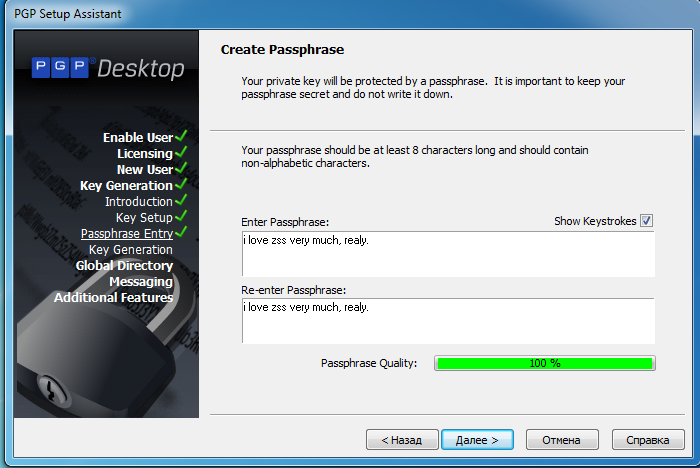
\includegraphics[scale=0.6]{pics/1.png}

        Рис. 1 – Создание кодовой фразы.
    \end{center}
    \begin{center}
        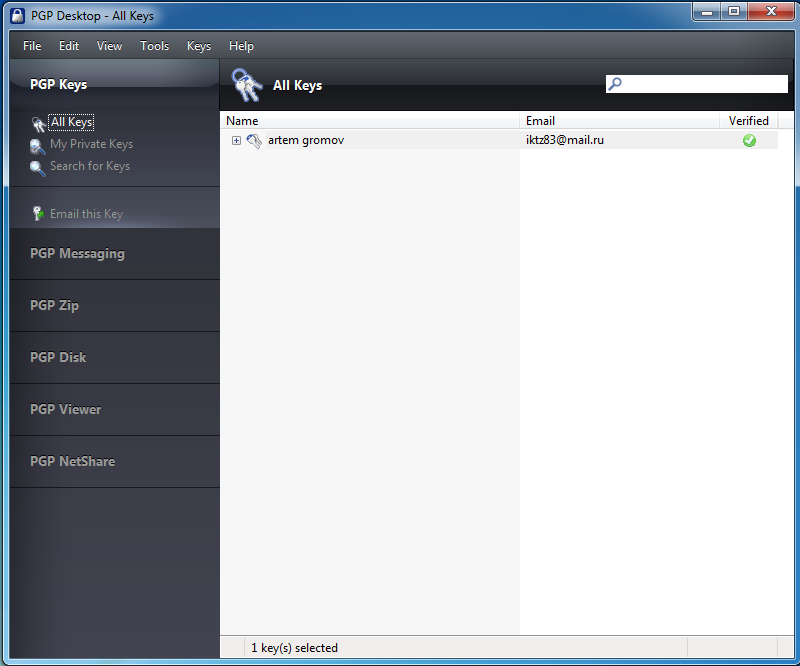
\includegraphics[scale=0.45]{pics/2.png}
        
        Рис. 2 – Ключи успешно созданы.
    \end{center}
    \begin{center}
        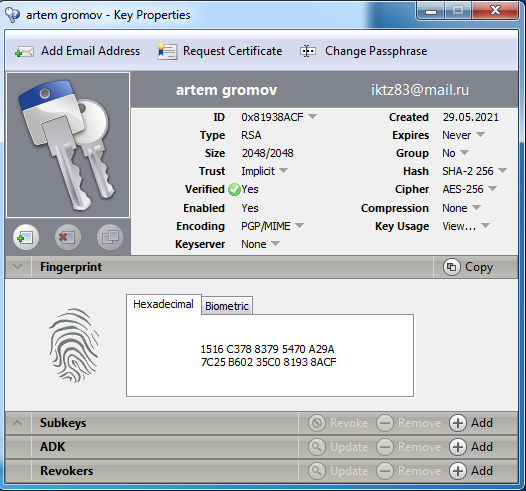
\includegraphics[scale=0.6]{pics/3.png}

        Рис. 3 – Проверка параметров ключа.
    \end{center}
    \begin{center}
        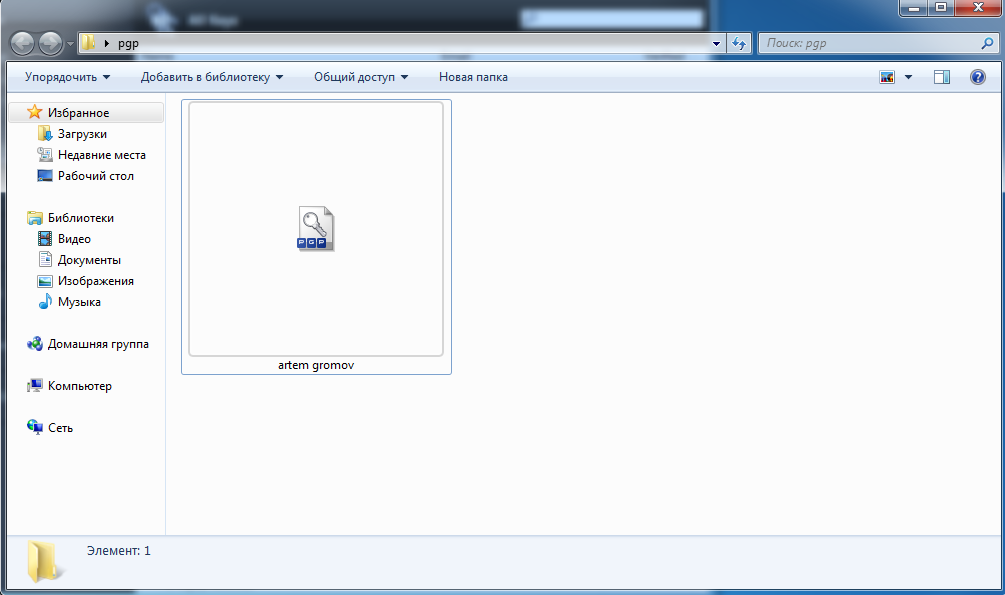
\includegraphics[scale=0.4]{pics/4.png}

        Рис. 4 – Экспорт ключа.
    \end{center}
    \begin{center}
        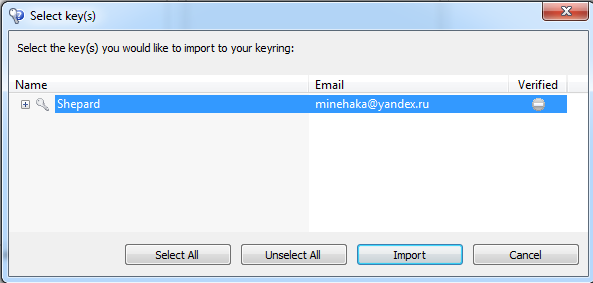
\includegraphics[scale=0.6]{pics/5.png}
        
        Рис. 5 – Импортируем ключ Георгия Урванцева.
    \end{center}
    \begin{center}
        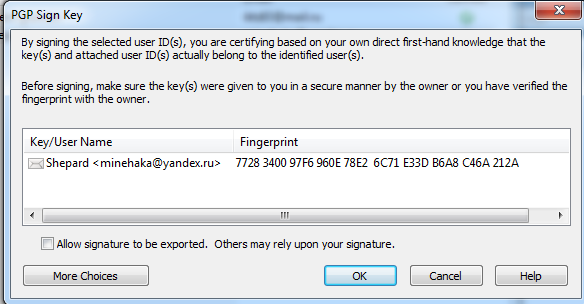
\includegraphics[scale=0.6]{pics/6.png}\\

        Рис. 6 – Подписываем пользователя(Георгия Урванцева).
        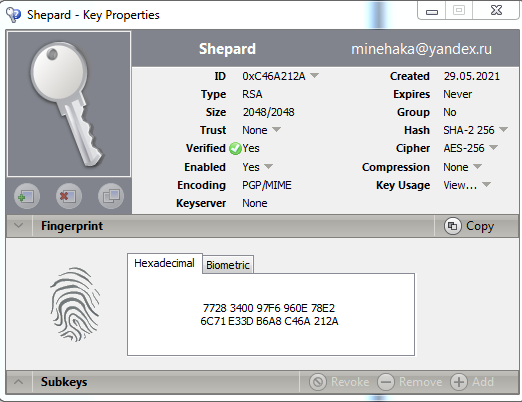
\includegraphics[scale=0.6]{pics/8.png}
        
        Рис. 7 – Проверка импортируемого ключа.
    \end{center}
    \begin{center}
        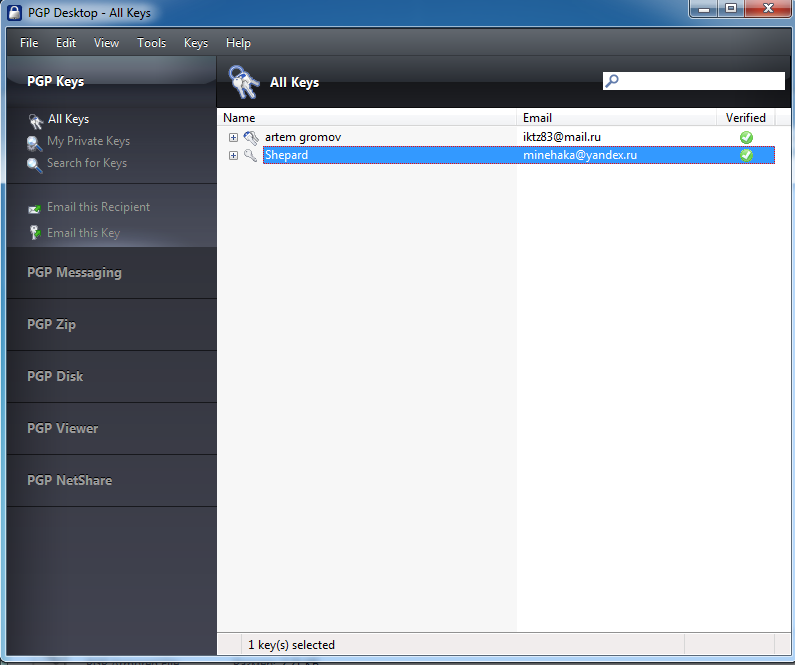
\includegraphics[scale=0.45]{pics/7.png}

        Рис. 8 – Ключ подписан успешно.
    \end{center}
    \begin{center}
        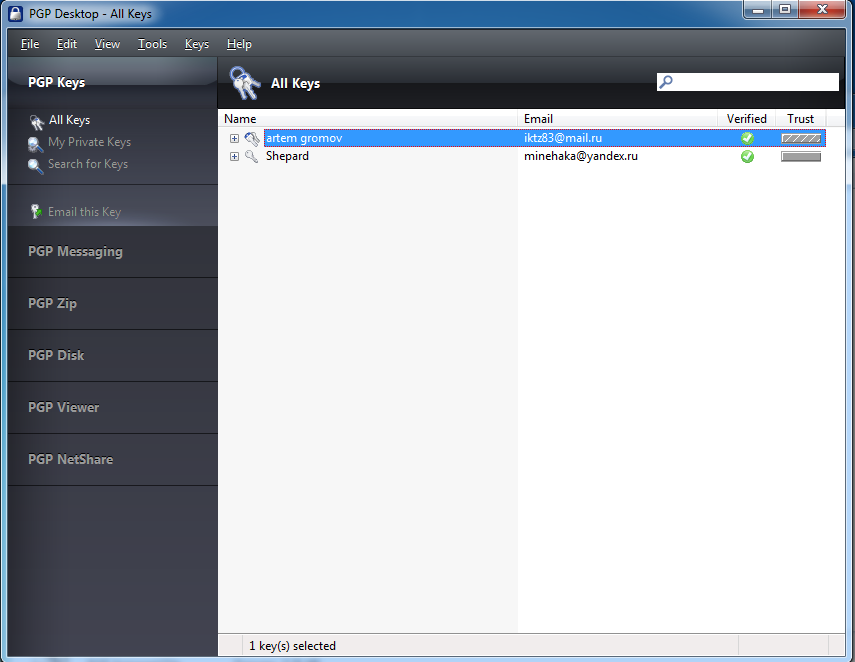
\includegraphics[scale=0.45]{pics/9.png}

        Рис. 9 – Уровня доверия установлен.
    \end{center}
    \begin{center}
        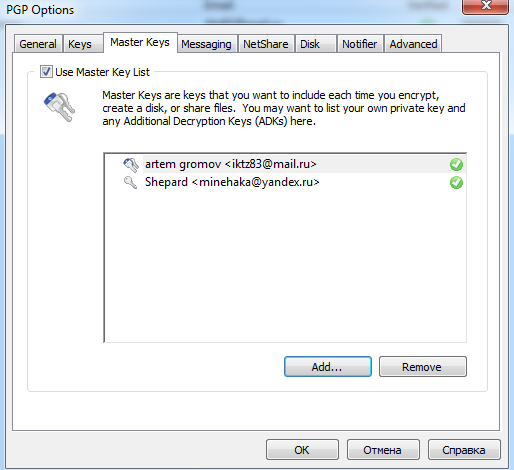
\includegraphics[scale=0.55]{pics/10.png}

        Рис. 10 – Добавление мастер-ключа
    \end{center}
    \begin{center}
        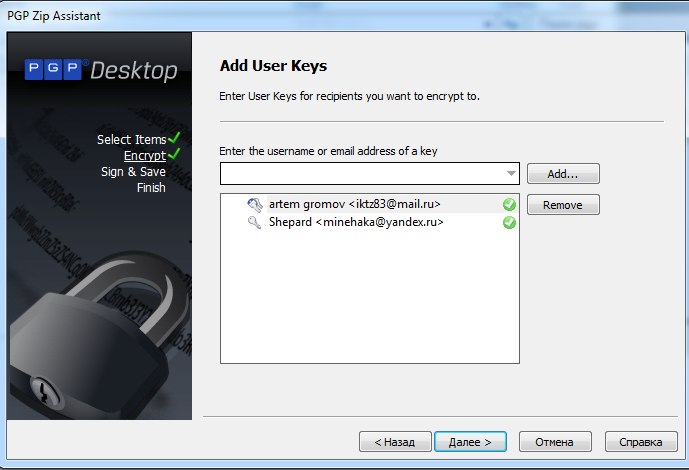
\includegraphics[scale=0.6]{pics/11.png}

        Рис. 11 – Зашифровка файла
        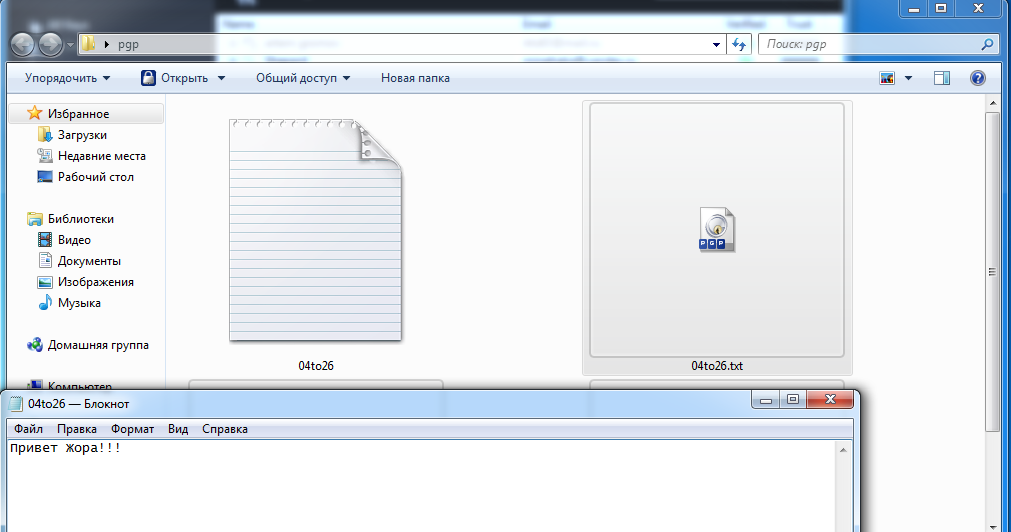
\includegraphics[scale=0.4]{pics/12.png}

        Рис. 12 – Зашифровка файла
    \end{center}
    \begin{center}
        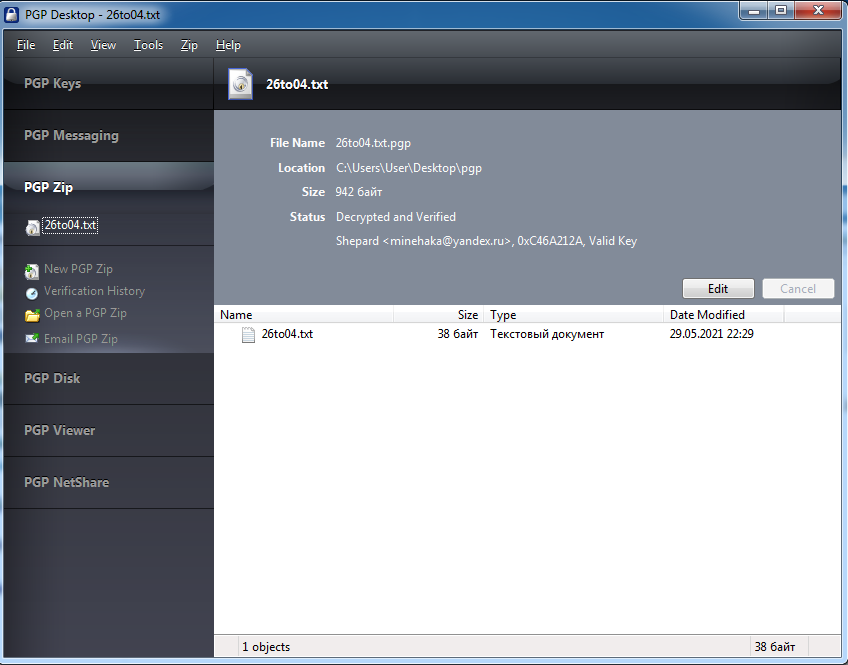
\includegraphics[scale=0.6]{pics/15.png}

        Рис. 13 – Расшифровка полученного от Георигия Урванцева файла
        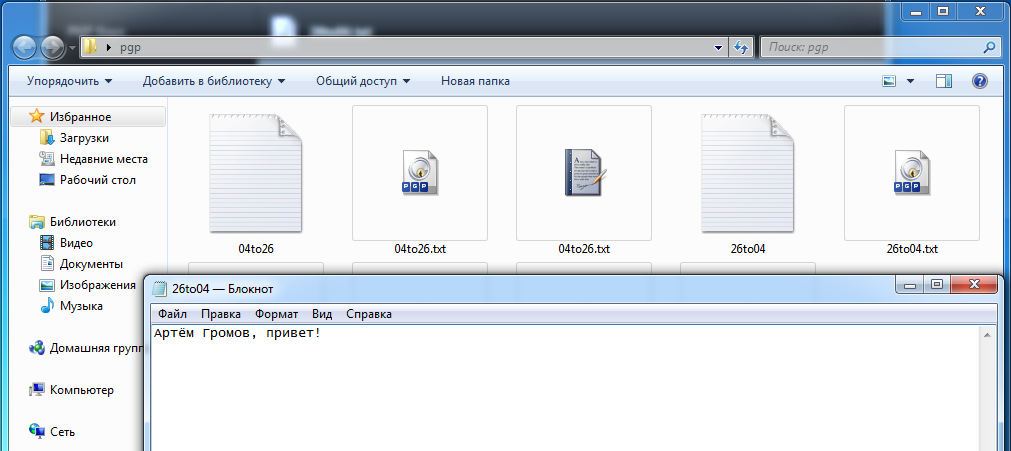
\includegraphics[scale=0.5]{pics/16.png}

        Рис. 14 – Расшифровка полученного от Георигия Урванцева файла
    \end{center}
    \begin{center}
        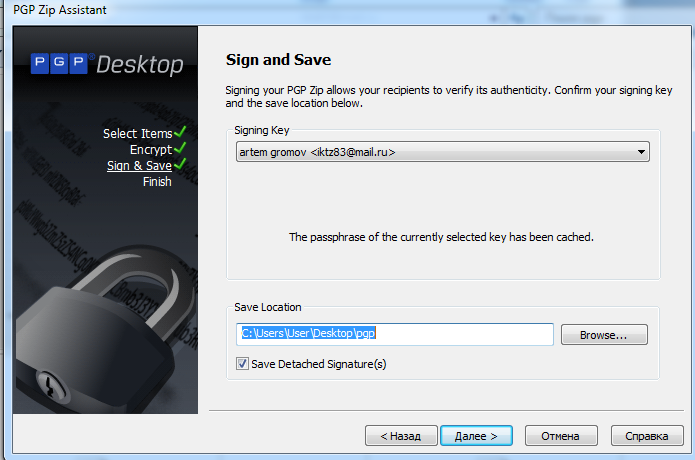
\includegraphics[scale=0.6]{pics/13.png}

        Рис. 15 – Подпись файла\\
        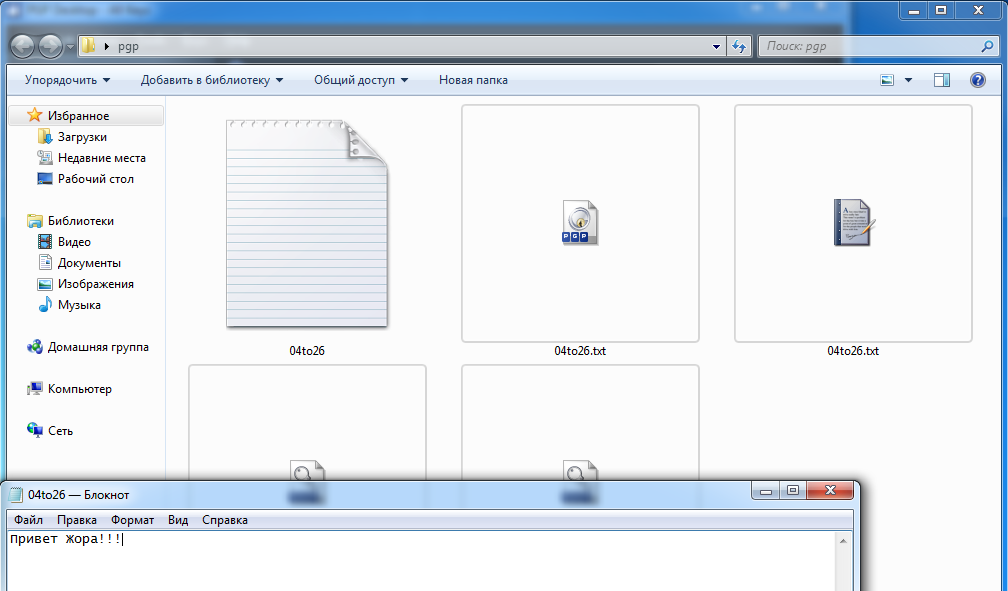
\includegraphics[scale=0.4]{pics/14.png}

        Рис. 16 – Подпись файла\\
        
\includegraphics[scale=0.7]{pics/17.png}
        
        Рис. 17 – Изначальный файл и файлы для Георгия Урванцева.
    \end{center}
    \begin{center}
        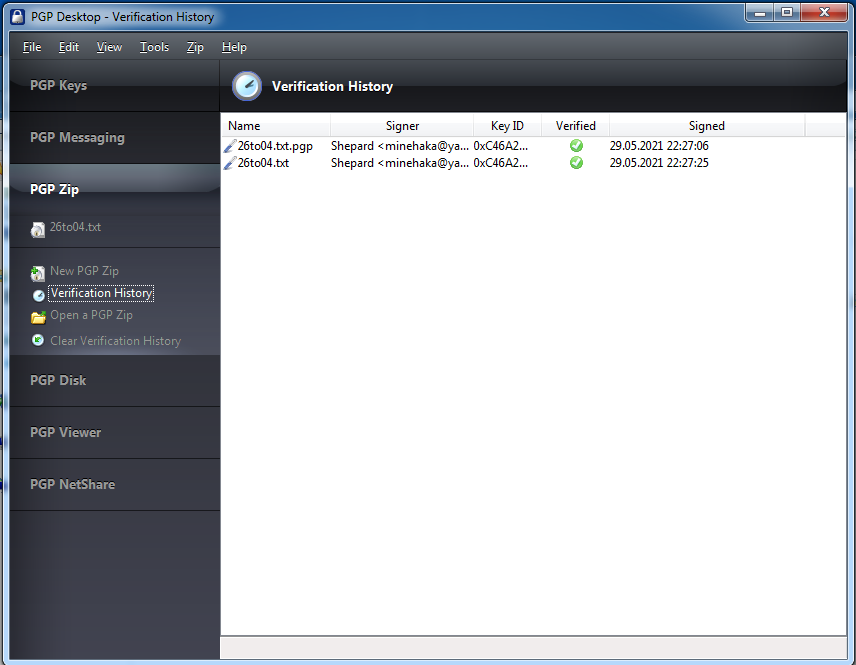
\includegraphics[scale=0.5]{pics/18.png}

        Рис. 18 – Проверка подписи полученного от Георгия Урванцева файла
    \end{center}
    \begin{center}
        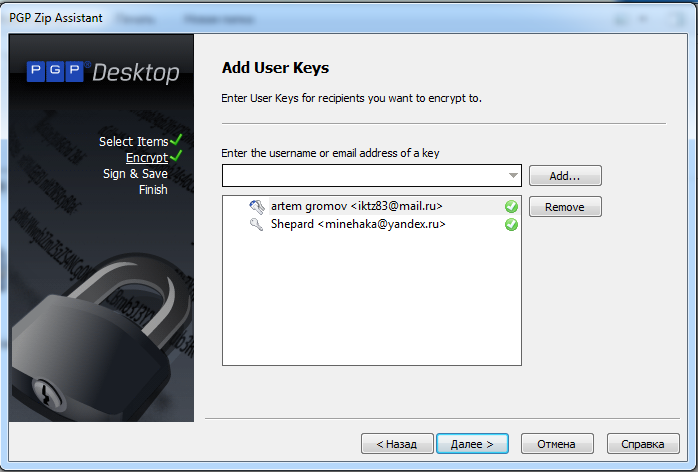
\includegraphics[scale=0.6]{pics/19.png}

        Рис. 19 – Создание подписанного и зашифрованного файла
    \end{center}
    \begin{center}
        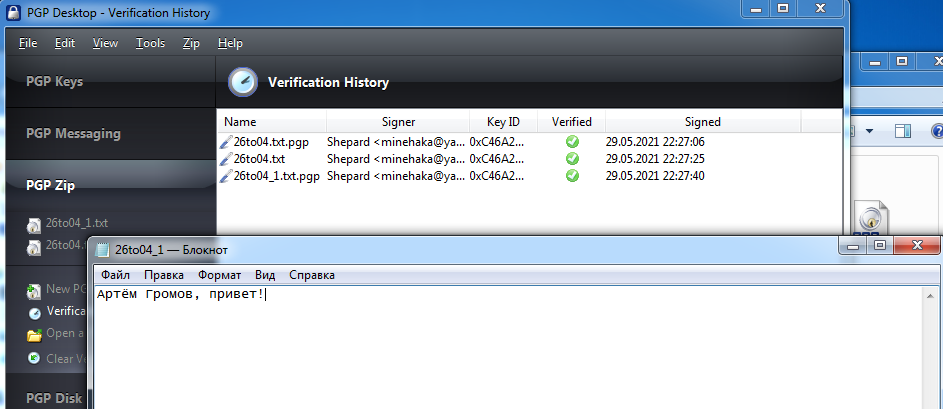
\includegraphics[scale=0.4]{pics/21.png}

        Рис. 20 – Файл успешно подписан и расшифрован
    \end{center}
    \textbf{Вывод:} \par
    В ходе данной лабораторной работы была изучен комплекс программ, включенных
    в PGP Desktop. С помощью данной программы были успешно подписаны и \linebreak 
    зашифрованы файлы. Обменявшись ключами и файлами, мы произвели проверку 
    подписи и расшифровку полученных файлов при обмене. Проверка прошла успешно.

\end{document}